\chapter{My first steps at HindSite, Inc. }

\section{Easy Web Content}

The first task I was given when arriving at HindSite Interactive was to get acquainted with their main application: Easy Web Content and especially with what is called the Easy Web Content Addons.

Easy Web Content is a web based software developed by HindSite Interactive. With it, users can easily manage their existing website: adding content, search engine optimizing, duplicate pages, ... Addons are specific complex content you can add to your pages : Photo Gallery, Calendar, Music Player, ... As the implementation of these addons was quite new in the software, some bugs were still existing. So I had to get familiar with the way they were built, to be able to resolve those bugs so that these addons could go live on the application. Previous interns had made a lot of documentation on them. It took me a week to read all the documentation and understand how they were built.

Also, the source code and user database information of these addons are located in another server than the one Easy Web Content runs in. So I also had to get familiar with the way the Easy Web Content server would communicate with the Addon Server to retrieve the information needed to handle these addons. That was pretty interesting as the communication uses a protocol I had never used before : SOAP \footnote{Simple Object Access Protocol}.


SOAP is a web service protocol that aims at exchanging structured information. It uses XML\footnote{eXtensible Markup Language} as its message format and RPC\footnote{Remote Procedure Call} or HTTP\footnote{HyperText Transfer Protocol} for its transmission. This protocol is based on three parts:
\begin{itemize}
\item The envelope, which defines what is in the message and how to process it
\item A set of encoding rules for expressing instances of application defined datatypes
\item A convention for representing procedure calls and responses
\end{itemize}
\lstset{language=XML}
\begin{lstlisting}[label=soap request,caption=Example of a SOAP request]
<?xml version="1.0"?>
<soap:Envelope
xmlns:soap="http://www.w3.org/2001/12/soap-envelope"
soap:encodingStyle="http://www.w3.org/2001/12/soap-encoding">

<soap:Body>
  <m:GetPrice xmlns:m="http://www.w3schools.com/prices">
    <m:Item>Apples</m:Item>
  </m:GetPrice>
</soap:Body>

</soap:Envelope>
\end{lstlisting}
\lstset{language=XML}
\begin{lstlisting}[label=soap response,caption=Example of a SOAP response]
<?xml version="1.0"?>
<soap:Envelope
xmlns:soap="http://www.w3.org/2001/12/soap-envelope"
soap:encodingStyle="http://www.w3.org/2001/12/soap-encoding">

<soap:Body>
  <m:GetPriceResponse xmlns:m="http://www.w3schools.com/prices">
    <m:Price>1.90</m:Price>
  </m:GetPriceResponse>
</soap:Body>

</soap:Envelope>
\end{lstlisting}
In this example, the client requested a web service called GetPrice, located at the url http://www.w3schools.com/prices. The SOAP server would execute the request, ie run the function GetPrice and return the response.

As it is XML based, SOAP is independent to whatever platform or programming language you are using. As an example, Easy Web Content server is using Java whereas the Addon server is using Php. Still, they are able to understand and handle the requests/responses that transit both ways.
The server that needs to retrieve the information is called a Soap Client. The one that provides the information is called the Soap Server. It provides what is called a Web Service. Any server around the world can retrieve the same information using this Web Service.

When I was fully acquainted with this protocol, I was able to create a new feature for Easy Web Content users: the creation of demo accounts. Users where now able to create demo accounts on Easy Web Site with the possibility to view addon presets so that they could get an overview of what they could do if they signed up for the complete version.


\section{A client project: Sencore}
After working on Easy Web Content, I was given the task to assist another developer in a huge client project for the company Sencore. The project's aim was to give the client a fully customized CMS\footnote{Content Management System} in which they could manage pretty much every aspect of their website, from customer requests, job applications to website content and product description. This project was my first real experience in Php/Mysql, and I was really excited about that.

The first task I achieved was the creation of a file uploader so that the client could upload their assets (images, pdf) to the website and then select from a list to incorporate them in the page.
\begin{figure}[!ht]
\centering
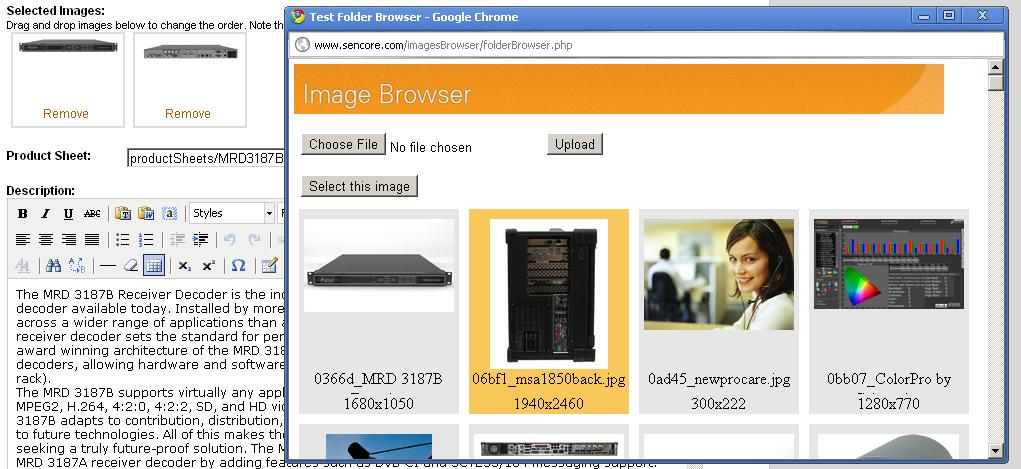
\includegraphics[width=.55\textwidth]{img/sencore.jpg}
\caption{Sencore File Uploaded}
\label{figure:sencore_uploader}
\end{figure}
\\The client can select from any image file on his computer and then upload it to the server. He will then directly see his image appear in the list underneath. Upon selection of the image, the popup will close and the image will be displayed in the appropriate content management section.

Then I created a "Print Page" functionality to allow customers to print the specification of a product. This task is basically achieved by changing the CSS of the html content you want to be printed: instead of setting width and padding of elements in pixels, you need to set it in percentage, a 100\% width meaning that the element will take the full width of a sheet of paper.

The last task I had to achieve in this project was not a development task. Unfortunately, sometimes the client will request you to do non development related stuff. This task consisted in populating all of their products in the Content management system, given pdf sheet they would give us. This was a really wearisome task as it meant doing the same thing over and over again for each of their products. I took me about a week to do so.
